\documentclass[12pt, twoside, openany]{book}
%chktex-file 1
%\documentclass[12pt, oneside]{book}  % jednostranna tlac
\linespread{1.25} % hodnota 1.25 by mala zodpovedat 1.5 riadkovaniu
\pagestyle{plain}
% -------------------
% --- Packages
% -------------------
\usepackage[a4paper,top=2.5cm,bottom=2.5cm,left=3.5cm,right=2cm]{geometry}
\usepackage[utf8]{inputenc}
\usepackage[T1]{fontenc}
\usepackage[slovak]{babel}
\usepackage{graphicx}
\usepackage{url}

% --- additional packages
\usepackage{epsfig}
\usepackage{epstopdf}
\usepackage[chapter]{algorithm}
\usepackage{algorithmic}
\usepackage{listings}
\usepackage{amsmath}
\usepackage{amssymb}
\usepackage{multirow}
\usepackage{booktabs}
\usepackage{color}
\usepackage{setspace}
\usepackage{tabularx}
\usepackage{textcomp}
\usepackage{caption}
\usepackage{natbib}
\usepackage{subcaption}
%\usepackage[font=large]{subcaption}
\usepackage{emptypage}
\usepackage{float}
\usepackage[hidelinks,breaklinks]{hyperref}
%\usepackage{minted}
\usepackage[thinlines]{easytable}
\usepackage{amsmath}
%\captionsetup[subfigure]{font=large}




%aby sa nevykreslovali obrazky
%\renewcommand{\includegraphics}[2][]{
%   \fbox{#2}% print file name in a small box
%}


% -------------------
% --- Definicia zakladnych pojmov
% -------------------
\def\mfrok{2024}
\def\mftitle{Automatická Generácia Úrovní pre Rytmické Počítačové Hry}
\def\mfthesistype{Diplomová práca}
\def\mfauthor{Bc. Filip Masný}
\def\mfskolitel{Ing. Viktor Kocur, PhD.}
\def\mfplacedate{Bratislava, 2024}
\def\mfuniversity{Univerzita Komenského v Bratislave }
\def\mffaculty{Fakulta matematiky, fyziky a informatiky}
\def\mfodbor{18. Informatika}
\def\program{Aplikovaná informatika}
\def\mfpracovisko{Katedra aplikovanej informatiky}

\begin{document}
\frontmatter


% -------------------
% --- Obalka ------
% -------------------
\thispagestyle{empty}

\noindent
\begin{minipage}{\textwidth}
    \begin{center}
        \textbf{\mfuniversity \\
            \mffaculty}
    \end{center}
\end{minipage}

\vfill
\begin{figure}[!hbt]
    \begin{center}
        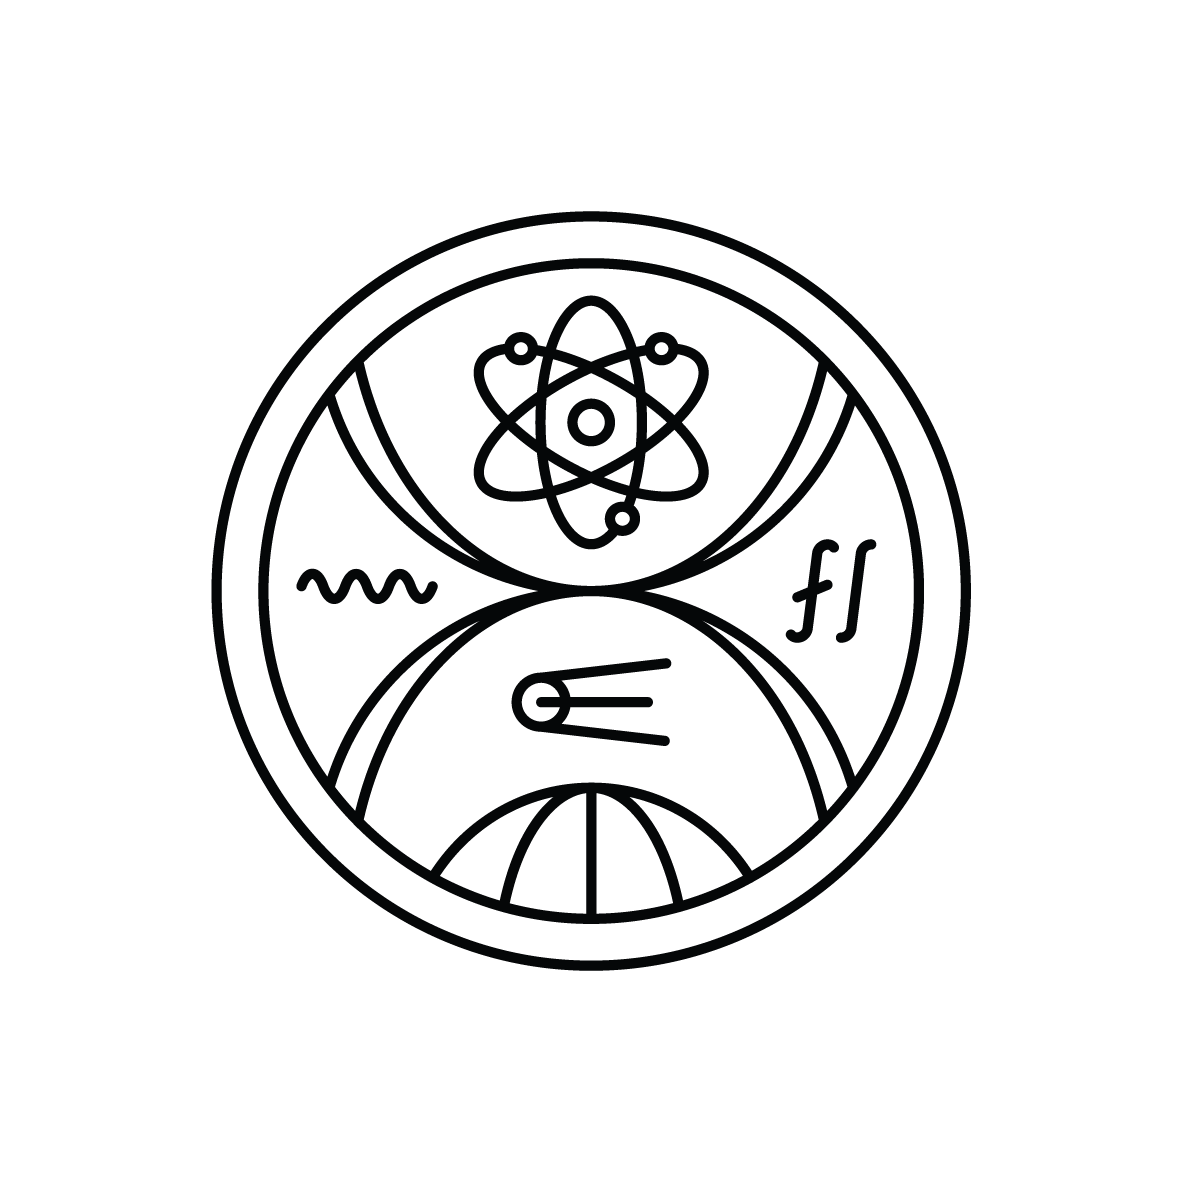
\includegraphics[width=0.4\textwidth]{images/FMFI_logo_BP.png}\label{img:logo}
    \end{center}
\end{figure}
\begin{center}
    \textbf{\MakeUppercase{\Large\mftitle}}\\
    \mfthesistype
\end{center}
\vfill
\mfrok \hfill
\mfauthor
%\eject 
\cleardoublepage
% --- koniec obalky ----



% -------------------
% --- Titulný list
% -------------------
\thispagestyle{empty}
\noindent
\begin{minipage}{\textwidth}
    \begin{center}
        \textbf{\mfuniversity \\
            \mffaculty}
    \end{center}
\end{minipage}

\vfill
\begin{figure}[!hbt]
    \begin{center}
        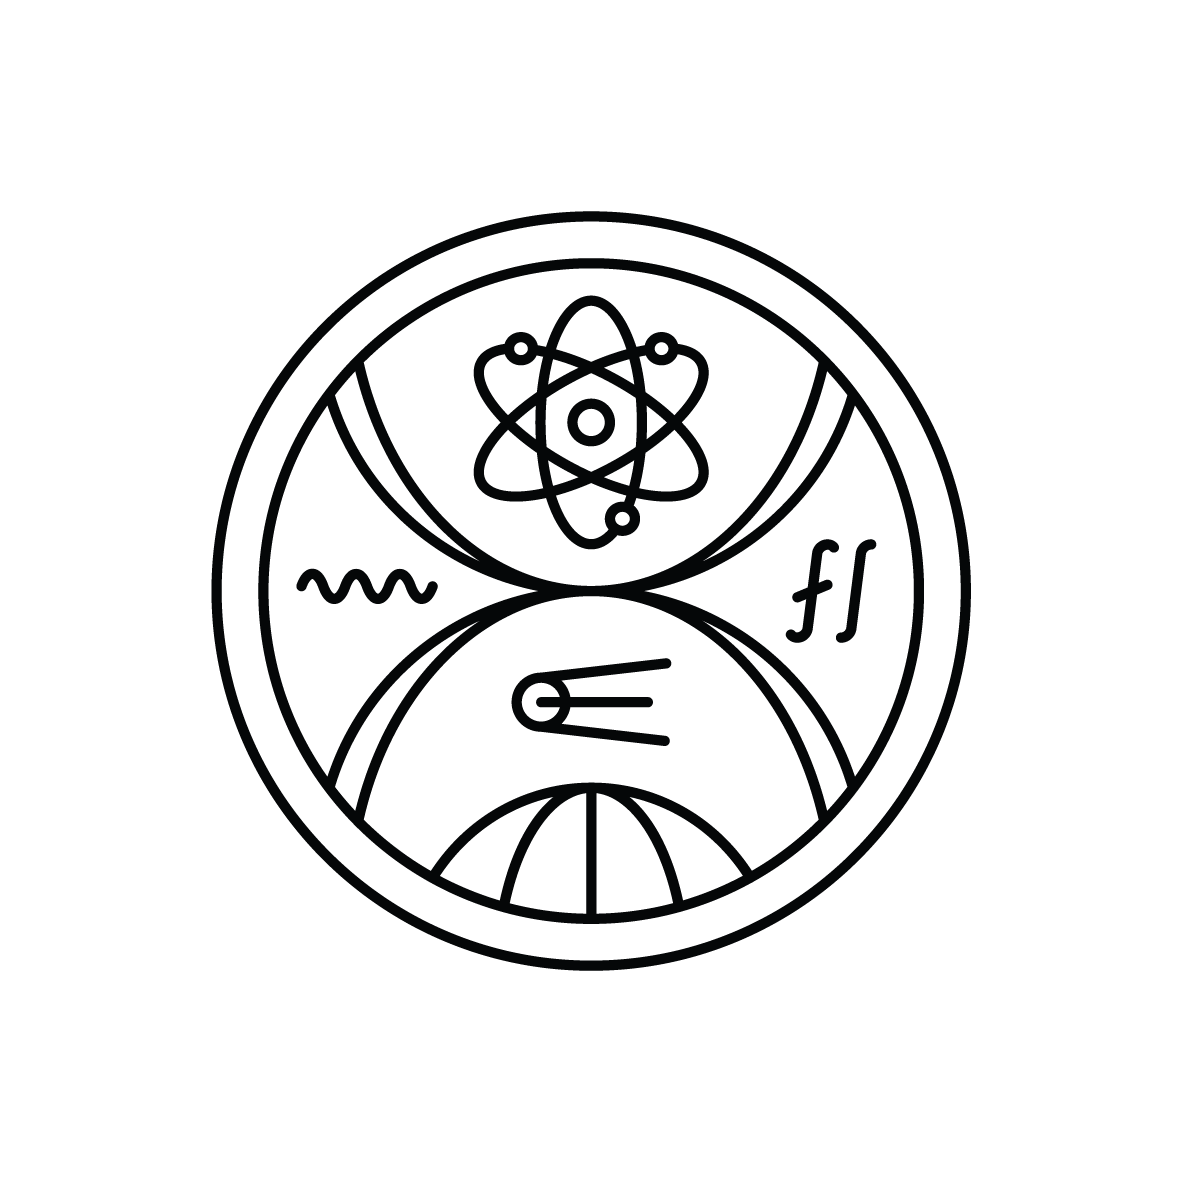
\includegraphics[width=0.4\textwidth]{images/FMFI_logo_BP.png}\label{img:logo_dark}
    \end{center}
\end{figure}

\begin{center}
    \textbf{\MakeUppercase{\Large\mftitle}}\\
    \mfthesistype
\end{center}
\vfill


\begin{tabular}{l l}
    Študijný program:    & \program      \\
    Študijný odbor:      & \mfodbor      \\
    Školiace pracovisko: & \mfpracovisko \\
    Školiteľ:            & \mfskolitel   \\
\end{tabular}

\vfill
\noindent
\mfplacedate \hfill
\mfauthor
%\eject 
\cleardoublepage
% --- Koniec titulnej strany



% -------------------
% --- Zadanie z AIS
% -------------------
% v tlačenej verzii s podpismi zainteresovaných osôb.
% v elektronickej verzii sa zverejňuje zadanie bez podpisov
% v pracach v naglictine anglicke aj slovenske zadanie

\newpage
\thispagestyle{empty}
%\hspace{-2cm}\includegraphics[page=1,width=1.1\textwidth]{zadaniePrace.PDF}

\newpage
\thispagestyle{empty}
%\hspace{-2cm}\includegraphics[page=2,width=1.1\textwidth]{zadaniePrace.PDF}

% --- Koniec zadania


% -------------------
% --- Prehlásenie
% -------------------

{~}\vspace{12cm}

\noindent
\begin{minipage}{0.25\textwidth}~\end{minipage}
\thispagestyle{empty}
\begin{minipage}{0.75\textwidth}
    Čestne prehlasujem, že túto diplomovú prácu som
vypracoval samostatne len s použitím uvedenej literatúry
a za pomoci konzultácií u môjho školiteľa.
\end{minipage}
\vfill
~\hfill {\hbox to 6cm{\dotfill}} \\
\mfplacedate \hfill \mfauthor
\vfill\eject \cleardoublepage
% --- koniec prehlasenia




% -------------------
% --- Poďakovanie
% -------------------
\newpage
\thispagestyle{empty}
\chapter*{Poďakovanie}\label{chap:thank_you}


\vfill\eject
% --- koniec podakovania


% -------------------
% --- Abstrakty
% -------------------
\newpage
\thispagestyle{empty}
\chapter*{Abstrakt}\label{chap:abstract_sk}
Rytmické počítačové hry predstavujú jedinečný žáner, kde hráči interagujú s hrou prostredníctvom preddefinovaných akcií synchronizovaných s hudobným sprievodom. Tieto akcie sú špecifikované v chart súboroch, ktoré sú obvykle vytvárané manuálnym úsilím skúsených umelcov známych ako chart artists. Táto práca sa zaoberá automatizáciou tohto procesu s cieľom demokratizovať tvorbu chartov a umožniť širšej verejnosti prispievať k tvorbe obsahu pre tieto hry.V rámci prehľadu tejto oblasti analyzujeme štruktúry chart súborov v populárnych rytmických hrách a preskúmame existujúce nástroje a literatúru súvisiacu s ich tvorbou. Na základe tejto analýzy navrhujeme a implementujeme algoritmus na automatizované vytváranie grafov, čím skracujeme proces tvorby a otvárame dvere pre nových tvorcov.Experimentálna časť práce sa zameriava na porovnanie kvality automaticky vytvorených chartov so chartami vytvorenými ľudskými umelcami. Na tento účel používame hodnotenia dobrovoľných hráčov, ktorí budú poskytovať spätnú väzbu na základe svojich herných skúseností. Týmto spôsobom hodnotíme efektivitu a presnosť nášho algoritmu voči manuálnej tvorbe.Výsledky tejto práce môžu prispieť k vývoju nových nástrojov na tvorbu obsahu pre rytmické hry a otvárať diskusiu o možnostiach automatizácie v tvorbe herného obsahu v iných žánroch.

\paragraph*{Kľúčové slová:}


\newpage
\thispagestyle{empty}
\chapter*{Abstract}\label{chap:abstract_en}
Rhythmic computer games rely on players executing predefined actions synchronized with accompanying music. These actions are specified in chart files, typically created manually by skilled artists known as chart artists. This work addresses the automation of this process to democratize chart creation and enable a broader community to contribute content to these games. Within the overview of this field, we analyze the structures of chart files in popular rhythmic games and explore existing tools and literature related to their creation. Based on this analysis, we propose and implement an algorithm for automated chart generation, streamlining the creation process and opening the door for new creators. The experimental part of the work focuses on comparing the quality of automatically generated charts with those created by human artists. For this purpose, we utilize evaluations from voluntary players who provide feedback based on their gaming experiences. This approach assesses the effectiveness and accuracy of our algorithm compared to manual creation. The results of this work can contribute to the development of new tools for content creation in rhythmic games and initiate discussions on the possibilities of automation in content creation across different gaming genres.

\paragraph*{Keywords:}


% --- koniec abstraktov


% -------------------
% --- Obsah
% -------------------
\newpage
\tableofcontents

% ---  Koniec Obsahu


% -------------------
% --- Zoznamy tabuliek, obrázkov - nepovinne
% -------------------
\newpage
\listoffigures
\listoftables
% ---  Koniec Zoznamov


\mainmatter


%main content 


% -------------------
% --- Bibliografia
% -------------------

\backmatter

\nocite{*}
\bibliographystyle{plain}
%\bibliography{references}

%---koniec bibliografie

\end{document}